\documentclass[hyperref={pdfpagelabels=false}]{beamer}
\let\Tiny=\tiny
\mode<presentation>{
\usetheme{Singapore}
%\usecolortheme{lily}
\usefonttheme{serif}
}
\usepackage{default}
%\usepackage{ucs}
\usepackage[utf8]{inputenc}
\usepackage{gb4e}
\usepackage[T1]{fontenc}
\usepackage{ tipa }
\usepackage{qtree}
\usepackage{synttree}
\usepackage{color}
\usepackage{tree-dvips}
\usepackage[absolute,overlay]{textpos}
%\usepackage{covington-beamer}
\usepackage{lmodern}
\usepackage{hyperref}
\usepackage{natbib}
\usepackage{graphicx}
\usepackage{eso-pic}
\usepackage{booktabs}
%\usepackage{memoir}
%\usepackage{relsize}
%\newcommand{\subscript}[1]{\raisebox{-0.25em}{\smaller #1}}
%\logo{\includegraphics[height=1cm]{nclcbelogomono.eps}}
\setbeamertemplate{footline}[frame number] 
%gets rid of navigation symbols
\setbeamertemplate{navigation symbols}{}

\title{Natural selection, language acquisition, and the specialization of variants over time}
\author{Joel C. Wallenberg\\\texttt{joel.wallenberg@ncl.ac.uk}}
\institute{
\includegraphics[scale = 0.2]{nclcbelogo.eps}}
\date[]{SUM-UP \\Potsdam Universität\\\vspace*{3mm}\url{www.staff.ncl.ac.uk/joel.wallenberg/papers/sumup_Wallenberg29June2018.pdf}}

\begin{document}

\begin{frame}[plain]
\titlepage
\end{frame}







\begin{frame}
\frametitle{Outline}
\tableofcontents
\end{frame}

\section{Specialization and Replacement}

\subsection{The Principle of Contrast and dimensions of specialization}

\begin{frame}
\frametitle{Diachronic Blocking Effect}
\begin{block}{``Blocking Effect'' \citep{aronoff1976}}
	\begin{itemize}
		\item General pressure against two forms existing for one function (``doublet''), forcing them to resolve in \textbf{replacement} or \textbf{specialization} \citep{kroch1994}.
		\item[ ]\{\textsl{lough, laughed}\} (laugh-\textsc{pst}; ME, \citealt{taylor1994})\\ \{\textsl{melted, molten}\} (PDE participle, adj pass)\\ \{\textsl{jimmies, sprinkles}\} (candy topping, Philadelphia)
		%\item The possible historical outcomes of a doublet are replacement (one form left) or specialization (forms diverge in function).
	\end{itemize}
\end{block}
\begin{block}{``Principle of Contrast''}
	\begin{itemize}
		\item A strategy that children use in acquiring language: assume that two forms have two meanings (or contexts)\citep[][{ \it inter alia}]{clark1987, clark1990}.
		\item Children hypothesize that novel words also refer to novel objects.
	\end{itemize}
\end{block}

\end{frame}






\begin{frame}
\frametitle{The Principle of Contrast (PrinCon)}
\begin{itemize}
	%\item A strategy that children use in acquiring language: assume that two forms have two meanings (or uses) (first stated in E. Clark 1987).
	\item Demonstrated in experiments such as \citet{markmanwachtel1988, bionetal2013}; see also nuanced review in \citet{bionetal2013}.
		\begin{enumerate}
			\item 20 children
			\item 6 pairs of one familiar item (banana, cow, cup, plate, saw, spoon) and one unfamiliar item (cherry pitter, odd shaped wicker container, lemon wedgepress, radish rosette maker, studfinder, tongs).
			\item \textbf{Control}: ``Show me one''
			\item \textbf{Test}: ``Show me the X'' (X = nonsense syllable)
		\end{enumerate}
	\item Control children pick the unfamiliar object at chance levels, but test children choose unfamiliar objects significantly higher than chance.
\end{itemize}
\end{frame}



\begin{frame}{...and observational results}
		\begin{exe}
			\ex Mo (at the fish-counter): That's a trout.\\
			 D (aged 2:5,1): That's a fish. That not a trout.\\
			 Mo: Well, a trout's a kind of fish.\\
			 D (pause, then pointing at a row of crabs): crabs are a kind of fish.\\
			 \citet[][97]{clark1995}
		\end{exe}
		
		
		
\end{frame}



\begin{frame}
\frametitle{Blocking = Contrast + Evolutionary Dynamics}
\begin{itemize}
	\item A doublet is two variants competing for finite resources (``competing grammars''), as in e.g. biological evolution.
		\begin{itemize} 
			\item Instead of competing for something like food, they are competing for use (time in the mouths/brains of speakers). 
			

			\end{itemize}
	\item Either one variant has a selectional advantage, and so \textbf{replaces} the other. 	
	\begin{itemize} \item \small{cf. \citet[][and subs.]{yang2000, yang2002}, \citet{heycockwallenberg2013}}

			\end{itemize}
	\item Or neither variant has an advantage (or much of one), in which case neutral change, drift (which can also lead to \textbf{replacement}; \citealt{kauhanen2016}).
	

	\item In language learning, the PrinCon means learners can pull apart the contexts of the variants, removing the competition through \textbf{specialization}.
\end{itemize}
\end{frame}


\begin{frame}{Example: Embedded Polar Questions}
		In all stages of English (and in historical Icelandic), a disjunction favors {\it whether} (\citealt{baileywallenbergwurff2012, wallenberg2016}, Wallenberg \textsl{in press})
	\begin{block}{English}
		\begin{itemize}
		\item[ ]\textbf{Disjunction:}
		\begin{exe}
			\ex I wonder \{{\bf whether},if\} John or Bill is bringing coffee.
			\ex I wonder \{{\bf whether},if\} John is bringing tea or coffee.
			%\ex I wonder \{whether,if\} John is bringing tea or not.
		\end{exe}
		\item[ ]\textbf{Simple:}
		\begin{exe}
			\ex I wonder \{whether, {\bf if}\} Bill is bringing coffee.
		\end{exe}
		\end{itemize}
	
	\end{block}
\end{frame}

\begin{frame}{Syntactic Variants}
\begin{exe}
	\ex \begin{xlist}
		\ex Mary wondered whether Sue was bringing coffee or not.
		\ex Mary wondered whether or not Sue was bringing coffee.
	\end{xlist}
	
	\ex \begin{xlist}
		\ex Mary wondered if Sue was bringing coffee or not.
		\ex * Mary wondered if or not Sue was bringing coffee.
	\end{xlist}
\end{exe}
\end{frame}

\begin{frame}{Slow Specialization of \textsl{whether/if} (N = 1929 clauses)} 


\begin{center}
 \small{Parsed Corpora: YCOE, PPCME2, PPCEME, PPCMBE \nocite{ycoe,ppcme2,ppceme,ppcmbe}}

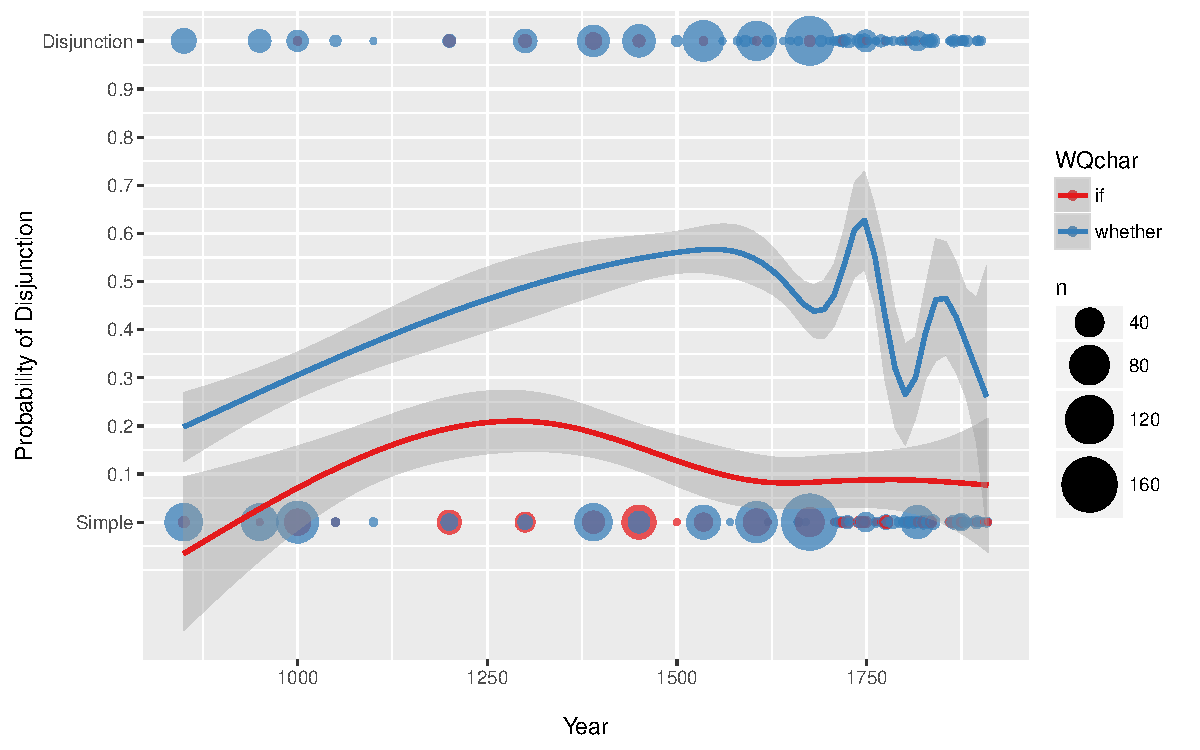
\includegraphics[width=1.1\textwidth]{whetherifEngDisjByYear.pdf}

\end{center}
\end{frame}

\begin{frame}{\textsl{whether/if} replacement slowed/arrested\\\small{(N = 1929 clauses)}}


%\begin{center}
 %\small{Parsed Corpora: YCOE, PPCME2, PPCEME, PPCMBE \nocite{ycoe,ppcme2,ppceme,ppcmbe}}

\includegraphics[width=1.1\textwidth]{whetherifEngWQByYearUnbinned.pdf}

%\end{center}
\end{frame}





\begin{frame}
\frametitle{Consequence: Blocking and Contrast}
\begin{itemize}
	\item A change can be:
		\begin{enumerate}
			\item A replacement change in progress (outright competition going to completion).
			\item A specialization change in progress (specialization for different functions).
			%\item \textbf{``Stable'' variation:} variants have \textbf{imperfectly specialized} along a continuous (or ordinal) dimension, e.g. style, prosodic weight. 
		\end{enumerate}
	\item If categorical variants specialize along a categorical dimension, complete specialization should eventually result.
	\item Specialization and replacement can happen simultaneously.
\end{itemize}

\end{frame}



\section{Morpho-lexical Case Study}
\subsection{How fast does specialization take place?}

\begin{frame}{Yang's Paradox?}
		\begin{center}
			Experimental results on word-learning show the Principle of Contrast differentiates words nearly instantaneously. The PrinCon is too fast to produce the slow specialization we see in, e.g. syntax. Is there another pressure?\\
			\vspace*{2mm}
			\small{(Caveat: \citet{bionetal2013} show retention of the new mapping is not instantaneous, and not reliable until after 24 months of age.)}\\
			\vspace*{5mm}
			\large{So, is it really true that word/morpheme specialization happens very quickly? And if not, what about the experimental evidence?}
		\end{center}
\end{frame}



\begin{frame}{\textsl{melted/molten} specialization}
\begin{itemize}
\item Variation in participle forms going back to OE: \textsl{gemolten, gemielted} (West Saxon), \textsl{gemælted} (Anglian), with the first adnominal use of \textsl{(ge-)molten} in 1300 (\textsc{melt}, OED).
\item \textsl{molten} in PDE now seems to be fully specialized (and maybe \textsl{melted} as well):
\end{itemize}
\begin{exe}
	\ex The gold was \{melted / *molten\} by the fire. \textbf{((passive) participle context)}
	\ex The fire has  \{melted / *molten\} the gold.\\\textbf{((past) participle context)}
	\ex The \{?melted / molten\} gold flowed down the hill. \textbf{(adjectival or adjectival passive DP-internal context)}
\end{exe}

\end{frame}

\begin{frame}{\textsl{melted/molten} specialization}
\begin{exe}
	\ex The gold was \{melted / *molten\} by the fire. \textbf{(participle context)}
	\ex The \{?melted / molten\} gold flowed down the hill. \textbf{(adjectival context)}
\end{exe}
\begin{itemize}
\item Question: how quickly did this morphological/lexical doublet specialize, in real time?

\item Question: how long did intraspeaker variation persist, in both contexts?
\item Using the {P}enn-{Y}ork {C}omputer-annotated {C}orpus of a {L}arge amount of {E}nglish based on the {TCP (PYCCLE-TCP; \citealt{pyccle})}, roughly 1 billion words.
\end{itemize}
\end{frame}


\begin{frame}{\textsl{melted/molten} specialization N =  7946 tokens}

%\begin{center}
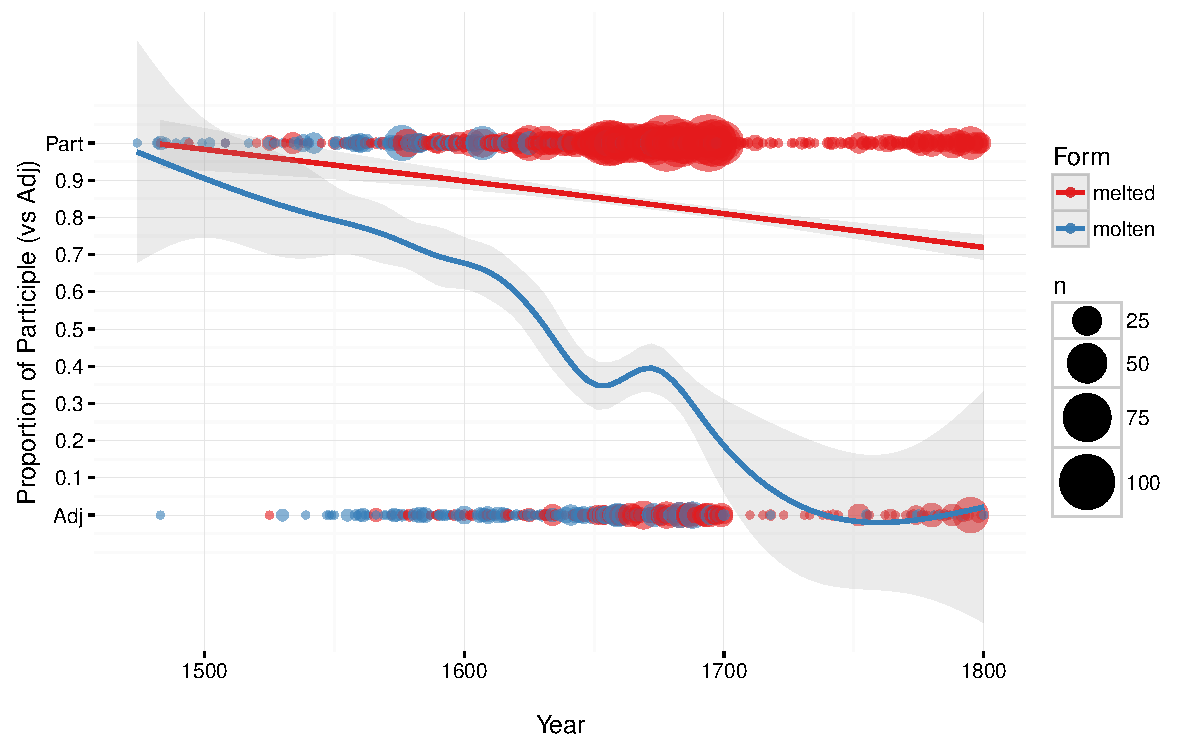
\includegraphics[width=1.128\textwidth]{ContextByDateUnbinnedWithDots2.pdf}
%\end{center}
\end{frame}


\begin{frame}{Simultaneous Replacement? N =  7946 tokens}

%\begin{center}
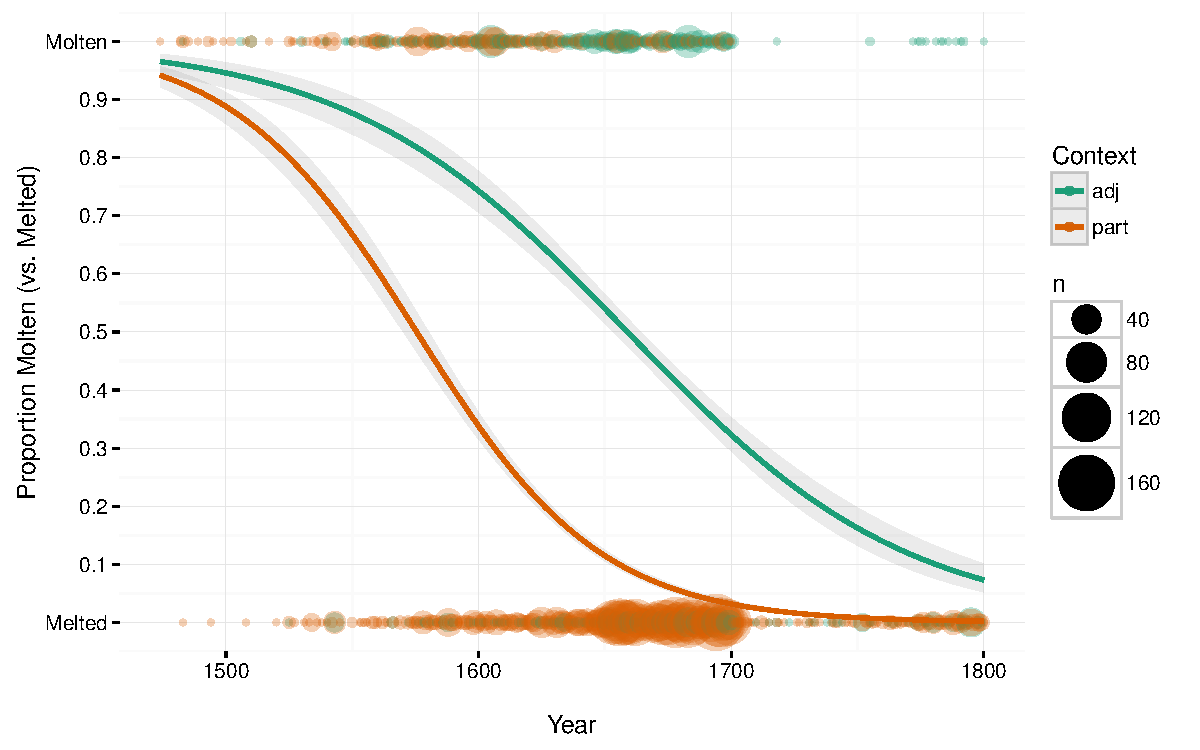
\includegraphics[width=1.128\textwidth]{FormByDateUnbinnedWithDots2.pdf}
%\end{center}
\end{frame}

\begin{frame}{Model Comparison: specialization by context}

\begin{center}
Model 1: Form \textasciitilde  (1 | file) + (1 | author) + zDate + Context\\
\vspace*{1mm}
Model 2: Form \textasciitilde  (1 | file) + (1 | author) + zDate{  }*{  }Context\\
\vspace*{4mm}

	\begin{tabular}{rrrr}
\toprule
	model & AIC & BIC & p-value (Chisq)\\
	\cmidrule{2-4}
Constant Rate & 4777.4 & 4812.3 & -- \\
with Date*Context &  4766.0 & 4807.8 & 0.0003\\
\bottomrule
\end{tabular}
\end{center}
\end{frame}



\begin{frame}{471 identifiable speakers, N = 3601 tokens}

%\begin{center}
%\small{(Note: the differing lengths of green lines, and 1575, 1580, 1601.)}
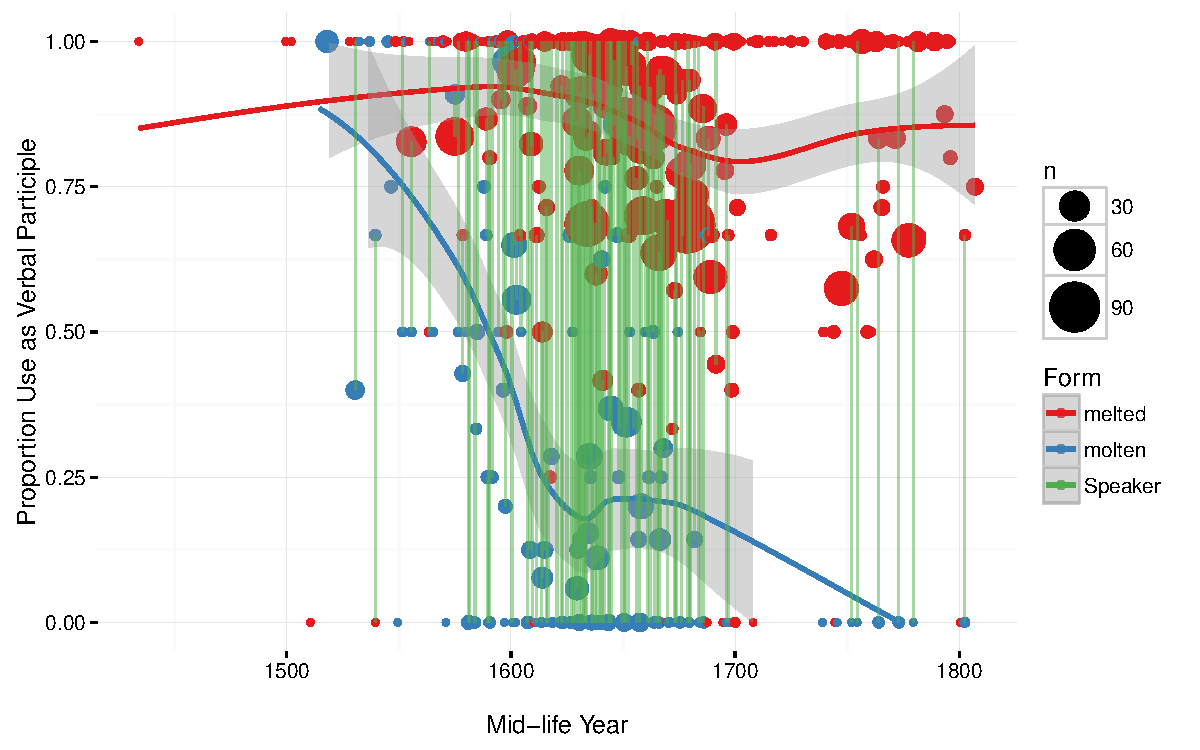
\includegraphics[width=1.128\textwidth]{ContextByDateAuthor.pdf}
%\end{center}%1575, 1601 for good variation, AND POINT OUT LENGTH OF GREEN LINE!
\end{frame}


\begin{frame}{Individual Speakers, 1570-1670 midlifes}

\begin{center}
\small{(Note: the differing lengths of green lines, and 1575, 1580, 1601)}

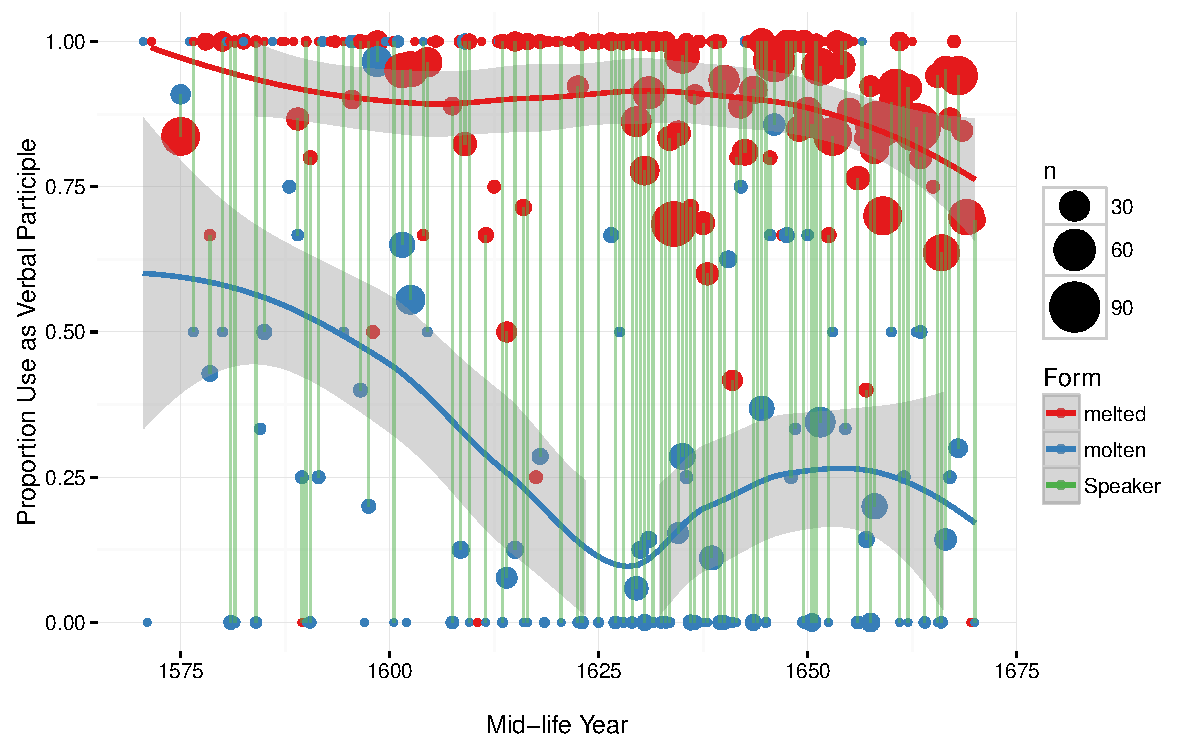
\includegraphics[width=1.128\textwidth]{ContextByDateAuthor1570.pdf}
\end{center}
%1575, 1601 for good variation, AND POINT OUT LENGTH OF GREEN LINE!
\end{frame}

\begin{frame}{Intraspeaker Variation}
		\begin{exe}
			\ex \begin{xlist} \ex Method of breeding Horses...Molten grease and fatning balls\\
			\ex ...which may bring away any melted grease\\
			\end{xlist}
			\ex \begin{xlist} \ex ...the grease is molten into them\\
			\ex ...considering that if grease should be melted\\
			\end{xlist}
			\ex \begin{xlist} \ex...adding thereto some Honey; which being molten , give it the Horse\\
			\ex ...English Honey; and when these are melted, and well stirred together\\
			\end{xlist}
		\end{exe}
		(Robert Almond, \textsl{The English horsman and complete farrier...}, date: 1673)
\end{frame}

\begin{frame}{Intraspeaker Variation}

\begin{center}
	Considering the 25 speakers who used > 5 tokens of both \textsl{molten} and \textsl{melted}:
\end{center}
\begin{itemize}
		\item None were fully specialized; none restricted one form to one context and the other to the other context.
	\item[] 13 (52\%) were \textbf{not} categorical in \textbf{either} form.
	\item[] 12 (48\%) were categorical in their use of one or other form.
	\item[] 19 (76\%) followed the community trend (i.e. PDE).
	\item[] 6 \hspace*{2mm}(24\%) showed the \textbf{opposite} pattern, with more \textsl{molten} in the participle contexts than \textsl{melted}.
	\item Shows a process of community coordination on the \textbf{direction} of specialization is taking place (perhaps in addition to the \textbf{dimension}).
\end{itemize}



\end{frame}


\begin{frame}{Solving Yang's Paradox}
		\begin{itemize}
			\item Perhaps the first generation to hear the innovation, Generation 1, does try to specialize completely.
			\item Generation 1 speakers will not necessarily converge on the same \textbf{dimension} of specialization (i.e. set of contexts), or the direction.
			\item Generation 2 cannot help but hear true synonyms, given the overlap of use in the community.
			\item Subsequent generations may converge on one dimension of specialization, but there will be intra- and inter-speaker variation along the way.
		\end{itemize}
\end{frame}


\section{Variational Specialization}
\subsection{Extending Yang (2000, 2002)'s model to specialization}


\begin{frame}{\citet{yang2000,yang2002}'s Variational Learner}
\begin{itemize}
	\item Children regularly entertain multiple hypotheses about some linguistic feature, say \textbf{Variant A} and \textbf{Variant B}.
	\begin{itemize}
		\item In times of change, both hypotheses may be valid; i.e. more than one variant for a parameter is present in the speech community.
		\item E.g. \textsl{shirt} is present, \textsl{skirt} is introduced; OV is present, VO is introduced; the speech community (and individuals) will use both interchangeably for a time, \textbf{and this must be learned}.
	\end{itemize}
	\item They track probabilities associated with each hypothesis, say $p$ for A and $(1-p)$ for B.
	\item Learners update the probabilities online as they encounter linguistic data.
\end{itemize}
\end{frame}


\begin{frame}{Specialization and Yang's Variational Learning}
		\begin{enumerate}
			\item Identify a domain of specialization:
				\begin{itemize}
					\item \textbf{Actively}, by the child innovating \textsl{de novo}?
					\item \textbf{Passively}, though random sampling of finite populations of utterances?
				\end{itemize}
			\item Allow the variants different (quantitative) representations for different contexts, along the domain of specialization:
			\begin{itemize}
				\item For categorical variants along categorical dimensions, decouple tracked frequencies of variants for each context, C_1,...,C_n, in the dimension of specialization.
			%	\item[\textcolor{blue}{b.}] For categorical variants along continuous dimensions, decouple tracked mean values (or targets) of variants for the dimension of specialization.
			\end{itemize}
			\item Specialization goes to completion as the learner has variants behave differently in different contexts.		\end{enumerate}
\end{frame}


\begin{frame}{3. Specialization completes}
\begin{itemize}
	\item Suppose Variant A is losing to Variant B due to global selective pressure, but they begin to specialize for C_1 and C_2.
	\item Specialization completes in a categorical dimension:
	\begin{itemize}
		\item \textbf{Actively}, by augmenting the represented frequency of Variant A in C_1 and augmenting Variant B in C_2?
		\item \textbf{Passively}, by allowing whatever evolutionary dynamics hold in the different contexts play out, whether the outcome is different or not?
	\end{itemize}
\end{itemize}
\end{frame}


\begin{frame}{Prediction for an Active Hypothesis}
		\begin{itemize}
			\item[] Once specialization begins to take place, it should be relentless, and \textbf{symmetrical}, and both variants should always survive.
				\begin{itemize}
					\item The frequency of Variant A in C_1 is always being augmented in lockstep with the punishment of Variant A in C_2. Both will have to survive, and:
					\begin{itemize}
					\item[\textbf{Corollary 1:}] the frequency of Variant A in C_1 and Variant A in C_2 will need to move away from each other.
					\item[\textbf{Corollary 2:}] the probability of C_1 being expressed by Variant A will rise as the probability of C_1 being expressed by Variant B declines.
					\end{itemize}
				\end{itemize}
		\end{itemize}
\end{frame}

\begin{frame}{\textsl{melted/molten}: consider Corollary 1}

%\begin{center}
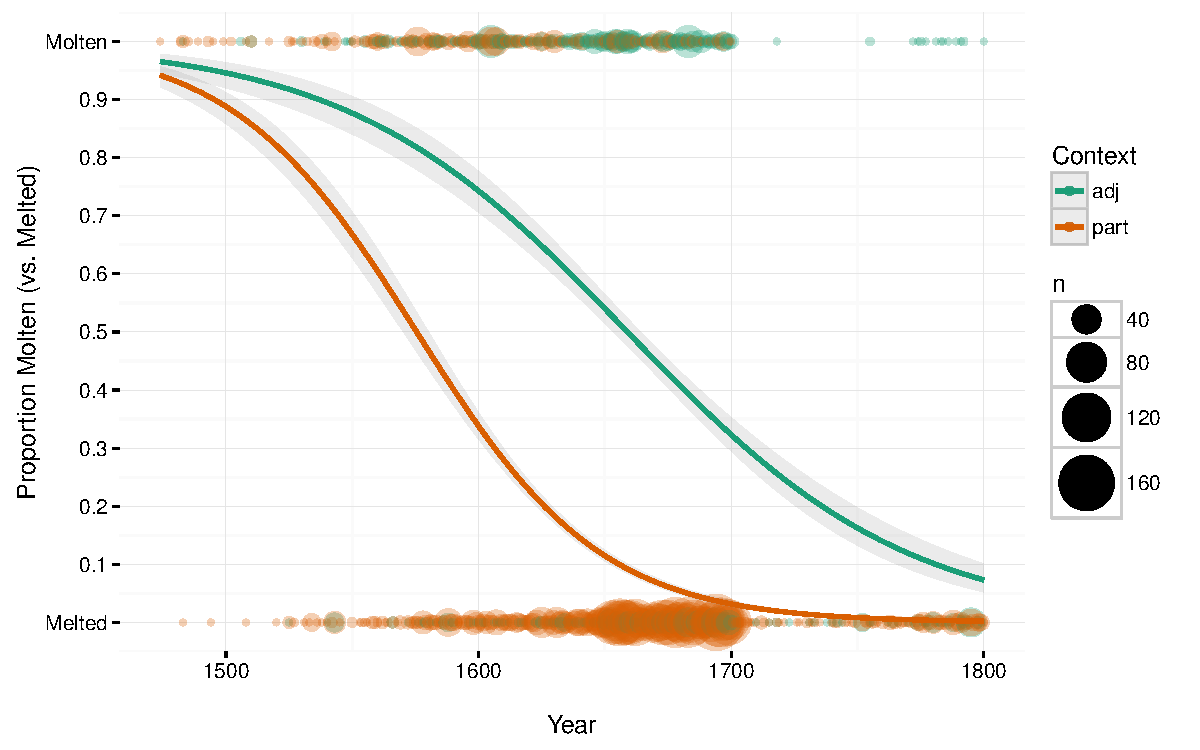
\includegraphics[width=1.128\textwidth]{FormByDateUnbinnedWithDots2.pdf}
%\end{center}
\end{frame}

\begin{frame}{\textsl{melted/molten}: consider Corollary 2}

\begin{center}
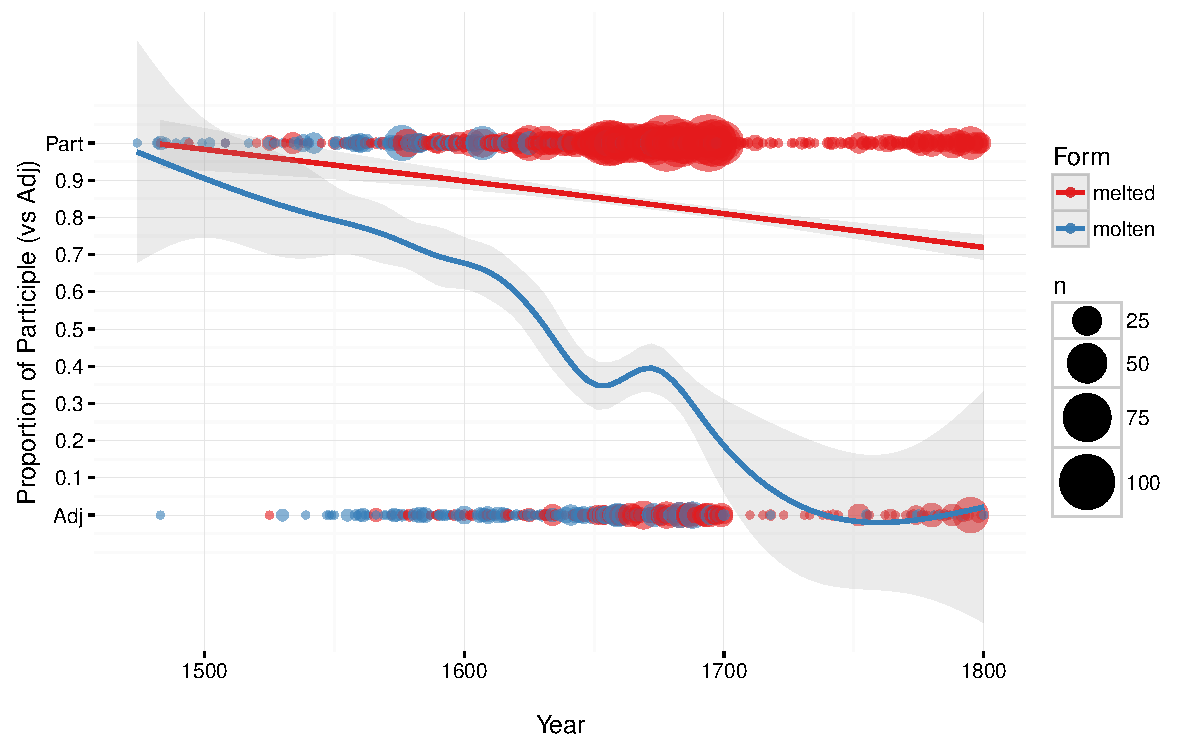
\includegraphics[width=1.128\textwidth]{ContextByDateUnbinnedWithDots2.pdf}
\end{center}
\end{frame}


\begin{frame}{Specialization in Acquisition: active or passive?}
		
		
		\begin{itemize}
			\item[ ] \textbf{Passive Hypothesis:} PrinCon \textbf{is} the decoupling of contexts C_1,...,C_n by learners, and the rest is due to the selective pressures being different in the different contexts, \textbf{once the tracked frequencies are decoupled in the learner's representation of the variation.}
			\begin{itemize} \item Distinguished from the Constant Rate Effect by the decoupling of the child's probability estimates for, e.g. Variant A in C_1,...,C_n.
			\item Contextual effects within the CRE can be thought of as transformations on a single tracked frequency for Variant A across all contexts.\end{itemize}
		\item Imagine a pond...	
		\end{itemize}
\end{frame}


\begin{frame}{Another Possible Pond Case}

\begin{center}
	Indefinite article allomorphs from the numeral \textsc{one}.
\end{center}
	
\begin{exe}
		\ex \begin{xlist} 
			\ex a table\\
			\ex an ear\\
			\end{xlist}
		\ex \begin{xlist} 
			\ex a tish\\
			\ex an eyer\\
			\end{xlist}
\end{exe}

\begin{center}
	\item Once \{a, an/eyn\} was innovated and the dimension of specialization chosen (following vowel)...
		\item \textsl{a} would have a cluster-avoiding advantage
	\item \textsl{an} would have a hiatus-avoiding advantage
\end{center}

\end{frame}

\begin{frame}{Another Possible Pond Case}
 
 \begin{exe}

 	\ex \textbf{Early Yiddish}
 	\begin{xlist} 
 		\ex \gll da iz eyn goyh kumn\\
 		there is a non-Jew-\textsc{fem} come\\
 		\ex  \gll a pritsh\\
 		a landowner-\textsc{fem}\\
 	\end{xlist}
 	\ex \begin{xlist}
 		 \ex \gll {der nakh} iz eyn {prits skts} kumin\\
 		 then is a landowner come\\
 		\end{xlist}
 	(1665 East Yiddish court cases, from \textsl{Penn Yiddish Corpus}, \citealt{santorini2008})
 \end{exe}  

   
  
  
\end{frame}

\begin{frame}{Another Possible Pond Case}

\begin{exe}
	\ex \textbf{Middle English}
	\begin{xlist} 
		\ex  a abbot\\
		\ex  a wrath fader\\
	\end{xlist}
	\ex \begin{xlist} 
		\ex \gll Loke what it is wrz þat ye ne sette an felun price þar-on\\
		Look what it is worth that you not set a deceitful price on-it\\
		\ex \gll Priuelike sal sho sende an ordane nunne\\
		Secretly shal she send an ordained nun\\
	\end{xlist}
	(\textsl{Northern Prose Rule of St. Benet,}, 1425, from  \textsl{Penn Parsed Corpus of Middle English 2}, \citealt{ppcme2})
\end{exe}  




\end{frame}




\section{Conclusion}

\begin{frame}{Conclusions}
		\begin{itemize}
			\item \textbf{Specialization} can allow competing forms to survive, but only if their functions diverge.
		%	\item \textbf{Imperfect specialization:} mismatch between categorical variation and continuous dimensions of specialization (or vice-versa) leads to long-term stochastic variation, though not quite stability.
			\item An extension of \citet{yang2000,yang2002}'s \textbf{variational learning model} provides some specific mathematical hypotheses about specialization in acquisition, which we can test.
			\item \textbf{PrinCon} has a natural definition in this model, and can be reconciled with the speed of specialization.
%			\item Two things I didn't discuss because of time:
			%\item The information on \textbf{transition} is based on very high-quality, expensive data (parsed diachronic corpora, beyond the ability of an individual to produce).%which allows us to observe a lot more than we could before.
			%\item It is still noisy, and we would like finer resolution as we tackle questions above, and e.g. selection vs. drift.
		\end{itemize}
\end{frame}



\begin{frame}{Final Conclusions and Challenges}
		\begin{itemize}
			\item Replacement and specialization both play out at an individual and speech community level, simultaneously.
			\item We can observe specialization diachronically, but can we observe the choosing of domains of specialization?
			\item Can we observe it in acquisition?
				\begin{itemize}
					\item Production data may not be good enough here.
				\end{itemize}
		\end{itemize}
\end{frame}


\begin{frame}{Acknowledgements}
\begin{center}
Thank you to Josef Fruehwald, Anthony Kroch, Betsy Sneller, Charles Yang. Special thanks to Aaron Ecay for help with PYCCLE and Weihnachtsgurke, among other things. Thanks also to Anton Karl Ingason, Laurel Mackenzie, and two anonymous reviewers.
\vspace{5mm}\\
\url{https://github.com/joelcw/molten}\\\vspace{3mm}

\includegraphics[scale = 0.1]{ncllogo.jpg} 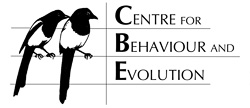
\includegraphics[scale = 0.4]{CBElogo.jpg} 
\end{center}
\end{frame}


\begin{frame}[allowframebreaks]
\frametitle{References}
\newcommand*{\newblock}{natbib}
\bibliographystyle{linquiry2}
\bibliography{joelrefs}
\end{frame}


\begin{frame}{Simultaneous replacement or extreme specialization?}
		\begin{exe}
			\ex \textbf{(\textsl{molten} implies heat in PDE:)}\\
			Is silly putty molten rubber?\\
			\ex \textbf{(\textsl{molten} implies liquidy/sludgy state in PDE:)}\\
			melted spatula vs. molten spatula\\
			\ex \textbf{(both:)}\\
			melted cheese vs. molten cheese\\
			(J. Fruehwald, p.c., for examples above)
			\ex \textbf{(\textsl{molten} implies recognizable substance in PDE:)}\\
			...that the increase and augmentation of Nilus commes of the snowe waters molten and thawed in those regions.\\
			(attr Barnabe Riche, \textsl{The famous hystory of Herodotus...}, date: 1584)
		\end{exe}
		
\end{frame}




\begin{frame}{3b. Specialization completes in the categorical-continuous case}
\begin{enumerate}
\item Suppose Variant A is losing to Variant B due to global selective pressure, but they begin to specialize along a continuous dimension C.
\item Learner allows their mean/target values for C to become distinct: $\mu$_{C_A},  $\mu$_{C_B}
\item Specialization completes in a continuous dimension:
\begin{itemize}
	\item \textbf{Actively}, by moving $\mu$_{C_A},  $\mu$_{C_B} away from each other?
	\item \textbf{Passively}, by allowing $\mu$_{C_A},  $\mu$_{C_B} the possibility of moving away from each other?
\end{itemize}
\end{enumerate}
\end{frame}


\begin{frame}{Specialization in Acquisition: active or passive?}
\begin{itemize}
	\item Is there any way to distinguish the two, given that different linguistic cases may have different selectional pressures?
	\begin{itemize}
		\item You can model a lot of scenarios assuming various selectional pressures interacting with various child-driven ``accelerations'' of specialization.
	\end{itemize}
	\item \textbf{Possible hypothesis:} maybe the child-driven amount of manipulating A and B's frequencies is the same per token in every linguistic case, and can be estimated.
	\item Maybe we can identify some true neutral changes, to abstract away from selective pressures \citep{kauhanen2016}.
\end{itemize}
\end{frame}



\begin{frame}{But what if there's a global selective pressure for B?}
		\begin{itemize}
			\item Once specialization begins to take place, it is relentless, but not necessarily symmetrical: if Variant A is losing globally, and C_1 and C_2 are decoupled, the amount of augmentation of Variant A in C_1 can be =, >, or < the global selective pressure against Variant A:			
			\begin{itemize}
					\item \textbf{amount of augmentation = selective pressure $\rightarrow$} variation is stable in C_1 and B wins in C_2.\\(THIS SCENARIO IS FULLY BIZARRE: we've now used the PrinCon to engineer stable variation.)
					\item \textbf{augmentation < selective pressure $\rightarrow$} Variant A loses in both C_1 and C_2 but at different rates.
					\item \textbf{augmentation > 2 x selective pressure $\rightarrow$} A wins in C_1 at the same rate B wins in C_2.
					\item \textbf{selective pressure < augmentation < 2 x selective pressure $\rightarrow$} A wins in C_1, but more slowly than B wins in C_2.			
			\end{itemize}
		\end{itemize}
\end{frame}






\begin{frame}{Phonological Specialization: \\ \small{GOOSE-NEW split in New Zealand English (Seyfarth and Sneller 2014)}}

\begin{center}
\includegraphics[width=.84\textwidth,height=.85\textheight]{../../../allophones/ByTokenOldPreceding.pdf}
\end{center}
\end{frame}


\begin{frame}{Spontaneous Phonologization: \\ \small{PRICE-raising in Philadelphia English (Fruehwald 2013)\\(308 speakers)}}

	
%\begin{center}
\includegraphics[trim=2cm 2cm 2cm 2cm, clip=false, width=.91\textwidth]{ayraisingphila.pdf}
%\end{center}

\end{frame}





\end{document}